% Sablon pentru realizarea lucrarii de licenta, conform cu recomandarile
% din ghidul de redactare:
% - https://fmi.unibuc.ro/finalizare-studii/
% - https://drive.google.com/file/d/1xj9kZZgTkcKMJkMLRuoYRgLQ1O8CX0mv/view

% Multumiri lui Gabriel Majeri, acest sablon a fost creat pe baza
% codului sursa a lucrarii sale de licenta. 
% Codul sursa: https://github.com/GabrielMajeri/bachelors-thesis
% Website: https://www.gabrielmajeri.ro/
%
% Aceast sablon este licentiat sub Creative Commons Attribution 4.0 International License.

\documentclass[12pt a4paper]{report}

%Enviroment nou pt a inlocui abstract din report
% \newenvironment{abstract}{
%     \chapter*{Abstract}
%     \addcontentsline{toc}{chapter}{Abstract}
%     \markboth{\MakeUppercase{Abstract}}{}
% }{
%     \clearpage
% }

\usepackage{times}

\usepackage{float}

% Suport pentru diacritice și alte simboluri
\usepackage{fontspec}

% Suport pentru mai multe limbi
\usepackage{polyglossia}

% Suport pentru enums
\usepackage{enumitem}

% Setează limba textului la română
\setdefaultlanguage{romanian}

% Am nevoie de engleză pentru rezumat
\setotherlanguages{english}

% Indentează și primul paragraf al fiecărei noi secțiuni
\SetLanguageKeys{romanian}{indentfirst=true}

% Font size
\fontsize{12}{14.4}\selectfont

% Suport pentru diferite stiluri de ghilimele
\usepackage{csquotes}

\DeclareQuoteStyle{romanian}
  {\quotedblbase}
  {\textquotedblright}
  {\guillemotleft}
  {\guillemotright}

% Utilizează biblatex pentru referințe bibliografice
\usepackage[
    maxbibnames=50,
    sorting=nty
]{biblatex}

\addbibresource{bibliography.bib}

% Setează spațiere inter-linie la 1.5
\usepackage{setspace}
\doublespacing

% Modificarea geometriei paginii
\usepackage{geometry}

% Include funcțiile de grafică
\usepackage{graphicx}
% Încarcă imaginile din directorul `images`
\graphicspath{{./images/}}

% Listări de cod
\usepackage{listings}

% Linkuri interactive în PDF
\usepackage[
    colorlinks,
    linkcolor={black},
    menucolor={black},
    citecolor={black},
    urlcolor={blue}
]{hyperref}

% Comenzi matematice
\usepackage{amsmath}
\usepackage{mathtools}

% Simboluri matematice codificate Unicode
\usepackage[warnings-off={mathtools-colon,mathtools-overbracket}]{unicode-math}

% Formule matematice
\newcommand{\bigO}[1]{\symcal{O}\left(#1\right)}
\DeclarePairedDelimiter\abs{\lvert}{\rvert}

% Suport pentru rezumat în două limbi
% Bazat pe https://tex.stackexchange.com/a/70818
\newenvironment{abstractpage}
  {\cleardoublepage\thispagestyle{empty}}
  {\vfill\cleardoublepage}
\renewenvironment{abstract}[1]
  {\cleardoublepage\bigskip\selectlanguage{#1}%
   \begin{center}\bfseries\abstractname\end{center}}
  {\par\bigskip}

% Suport pentru anexe
\usepackage{appendix}

% Stiluri diferite de headere și footere
\usepackage{fancyhdr}

% Mutam textul de la capitole putin mai la dreapta
\usepackage{tocloft}
\cftsetindents{chapter}{-0.5em}{2.5em} % primul e pt distanta cifrei fata de margine, a doua e pt distanta dintre cifra si litera
\cftsetindents{section}{1em}{3em}

% Metadate
\title{Proiectarea și implementarea arhitecturilor chatbot cu aplicații în industria bancară}
\author{Andriță Lucian-Gabriel}

% Generează variabilele cu @
\makeatletter

\begin{document}

% Front matter
\cleardoublepage
\let\ps@plain

% Coperta
\begin{titlepage}

% Redu marginile
\newgeometry{left=2cm,right=2cm,bottom=1cm}

\begin{figure}[!htb]
    \centering
    \begin{minipage}{0.2\textwidth}
        
\includegraphics[width=\linewidth]{logo-ub.png}
    \end{minipage}
    \begin{minipage}{0.5\textwidth}
        \large
        \vspace{0.2cm}
        \begin{center}
            \textbf{UNIVERSITATEA DIN BUCUREȘTI}
        \end{center}
        \vspace{0.3cm}
        \begin{center}
            \textbf{
                FACULTATEA DE \\
                MATEMATICĂ ȘI INFORMATICĂ
            }
        \end{center}
    \end{minipage}
    \begin{minipage}{0.2\textwidth}
        
\includegraphics[width=\linewidth]{logo-fmi.png}
    \end{minipage}
\end{figure}

\begin{center}
\textbf{SPECIALIZAREA TEHNOLOGIA INFORMAȚIEI}
\end{center}

\vspace{4cm}

\begin{center}
\huge \textbf{\MakeUppercase{Lucrare de licență}}
\end{center}

\vspace{3cm}

\begin{center}
\large \textbf{Absolvent \\ \@author}
\end{center}

\vspace{0.25cm}

\begin{center}
\large \textbf{Coordonator științific \\ Prof. dr. Cristian Kevorchian}
\end{center}

\vspace{2cm}

\begin{center}
\Large \textbf{București, iunie 2023}
\end{center}
\end{titlepage}

% Pagina de titlu
\begin{titlepage}

% Redu marginile
\newgeometry{left=2cm,right=2cm,bottom=1cm}

\begin{figure}[!htb]
    \centering
    \begin{minipage}{0.2\textwidth}
        
\includegraphics[width=\linewidth]{logo-ub.png}
    \end{minipage}
    \begin{minipage}{0.5\textwidth}
        \large
        \vspace{0.2cm}
        \begin{center}
            \textbf{UNIVERSITATEA DIN BUCUREȘTI}
        \end{center}
        \vspace{0.3cm}
        \begin{center}
            \textbf{
                FACULTATEA DE \\
                MATEMATICĂ ȘI INFORMATICĂ
            }
        \end{center}
    \end{minipage}
    \begin{minipage}{0.2\textwidth}
        
\includegraphics[width=\linewidth]{logo-fmi.png}
    \end{minipage}
\end{figure}

\begin{center}
\textbf{SPECIALIZAREA TEHNOLOGIA INFORMAȚIEI}
\end{center}

\vspace{1cm}

\begin{center}
\Large \textbf{Lucrare de licență}
\end{center}

\begin{center}
\huge \textbf{\MakeUppercase{\@title}}
\end{center}

\vspace{3cm}

\begin{center}
\large \textbf{Absolvent \\ \@author}
\end{center}

\vspace{0.25cm}

\begin{center}
\large \textbf{Coordonator științific \\ Prof. dr. Cristian Kevorchian}
\end{center}

\vspace{2cm}

\begin{center}
\Large \textbf{București, iunie 2023}
\end{center}
\end{titlepage}
\restoregeometry
\newgeometry{
    margin=2.5cm
}

\fancypagestyle{main}{
  \fancyhf{}
  \renewcommand\headrulewidth{0pt}
  \fancyhead[C]{}
  \fancyfoot[C]{\thepage}
}

% Rezumatul
\pagestyle{empty}
\begin{abstractpage}

\begin{abstract}{romanian}

Acesta este un șablon C++ care utilizează Dialogflow ES de la Google Cloud Platform pentru interacțiuni între oameni și chatbot în diferite contexte, în funcție de cazurile de utilizare ale întreținătorului. Această aplicație în particular folosește procesarea în cloud într-un context bancar și a fost creată ca o dovadă a unui concept, obiectivul principal fiind de a-mi extinde cunoștințele cu privire la interacțiunile C++ într-un mediu modern, utilizând diferite servicii cloud pentru a izola funcționalitățile principale ale aplicației, mutând implementarea locală într-una găzduită în cloud. 

Serverul care gestionează conexiunea între clienți și agent este găzduit local. Atunci când se primește o solicitare de la un client, serverul decide ce tip de fișiere să trimită. Pe măsură ce clientul își face interogari către agent, un script va acționa ca parser pentru textul dat și va asculta răspunsul de la server. Când serverul primește intrarea, o va trimite la agent. În cloud, agentul va potrivi textul primit cu o intenție, va extrage unii parametrii în funcție de intenție și va apela un webhook. Webhook-ul constă într-o funcție Google Cloud Function, care este găzduită pe Google Source Repository, unde va căuta în dosarul cloud și va extrage funcționalitatea de acolo. 

Funcția va avea privilegii CRUD+L asupra unui bucket Google Cloud Storage care stochează informațiile necesare. Acest studiu reprezintă o contribuție semnificativă la înțelegerea modului în care serviciile de cloud pot fi integrate cu succes în aplicațiile bazate pe C++, cu un accent specific pe dezvoltarea chatbot-urilor în industria bancară.
\end{abstract}

\begin{abstract}{english}

This is a C++ template that uses Google Cloud Platform's Dialogflow ES for human-chatbot interactions in different contexts, depending on the use cases of the maintainer. This particular application uses cloud processing in a banking context and was created as a proof of concept, its main goal being to further expand my knowledge regarding C++ interactions in a modern enviroment, while using different cloud services to isolate main functionalities of the application moving the local implementation to a cloud hosted one. 

The server that is serving the connection between the clients and the agent is locally hosted. When a request from a client is received, the server decides what type of files to send. As the client queries his intent to the agent, a script will act as a parser for the given text, and will listen for the response from the server. When the server receives the input, it will send it to the agent. In the cloud, the agent will match the received text with an intent, it will extract some parameters based on the intent, and it will call a webhook. The webhook consists of a Google Cloud Function, that's being hosted on Google Source Repository, where it will look into the cloud folder and extract the functionality from there. 

The function will have CRUD+L privileges on a Google Cloud Storage bucket that stores the needed information. This study represents a significant contribution to the understanding of how cloud services can be successfully integrated into C++ based applications, with a specific focus on the development of chatbots in the banking industry.
\end{abstract}

\end{abstractpage}

\addtocounter{page}{1}

% Modificare pentru cuprins
\pagestyle{empty}
\tableofcontents
\renewcommand{\thechapter}{\Roman{chapter}} % Chapter numbering: I, II, III, etc.
\renewcommand{\thesection}{\thechapter.\arabic{section}} % Section numbering: 1, 2, 3, etc.
\renewcommand{\thesubsection}{\thesection.\arabic{subsection}} % Subsection numbering: 1.1, 1.2, 2.1, 2.2, etc.
\renewcommand{\thesubsubsection}{\thesubsection.\arabic{subsubsection}} % Subsubsection numbering: 1.1.1, 1.1.2, 2.1.1, 2.1.2, etc.

% Main matter
\cleardoublepage
\pagestyle{main}
\let\ps@plain\ps@main

\chapter{Introducere}

\section{Nevoia migrării în cloud}

În era digitală modernă, tendința de procesare mutată în cloud a devenit o parte integrală a multor domenii și industrii. Această tendință se referă la transferul și executarea operațiunilor de procesare a datelor și sarcinilor complexe în cloud, în loc să fie realizate local.

Procesarea mutată în cloud oferă o abordare inovatoare și scalabilă pentru gestionarea volumelor mari de date și sarcini computaționale intensive. Prin intermediul infrastructurii cloud, această tendință permite accesul la resurse computaționale puternice și flexibile, oferind astfel utilizatorilor o experiență îmbunătățită și performanțe superioare în timp real \cite{benefits-of-cloud-computing}.

Prin transferarea sarcinilor în mediul cloud, utilizatorii beneficiază de o serie de avantaje. Unul dintre acestea este accesul la capacități de procesare și resurse de stocare extinse, care pot depăși de multe ori puterea de calcul a dispozitivelor individuale. Această scalabilitate permite utilizatorilor să gestioneze sarcini complexe, cum ar fi analiza unor seturi de date foarte mari, procesarea grafică avansată sau algoritmi de învățare automată, fără a se confrunta cu constrângerile tehnice ale dispozitivelor personale.

Pe lângă avantajele de performanță, procesarea mutată în cloud oferă și o mai mare flexibilitate și mobilitate. Utilizatorii pot accesa și gestiona datele și aplicațiile lor de pe diferite dispozitive, indiferent de locație sau de sistemul de operare utilizat. Acest aspect aduce un nivel crescut de colaborare și sincronizare între utilizatori, sporind eficiența și productivitatea în mediul de lucru modern.

Totuși, pe lângă beneficiile pe care le aduce, procesarea mutată în cloud aduce anumite provocări și preocupări. Una dintre ele este legată de securitatea datelor și confidențialitatea informațiilor. Deoarece datele sunt transferate și procesate în mediul cloud, există riscul ca acestea să fie expuse la amenințări cibernetice sau să fie accesate de persoane neautorizate. Drept urmare, furnizorii de servicii cloud trebuie să implementeze măsuri solide de securitate și criptare pentru a proteja datele utilizatorilor.

\section{Scopul lucrării}

Aplicația este un template care îmbină procese moderne de prelucrare și stocare a datelor folosind servicii cloud. Scopul acesteia este de a fi o implementare practică a unui concept și de a-mi îmbunătăți cunoștiințele cu privire la servicii cloud, arhitectură de aplicații, limbajul C++, clean coding, precum și best practices în acest context. Codul sursă se poate găsi pe pagina personală de GitHub \cite{github}.

Alegerea unui limbaj precum C++ pentru dezvoltarea unei aplicații web a prezentat o provocare în ceea ce privește alegerea utilitarului potrivit pentru crearea și gestionarea serverului. Multe aplicații întâlnite folosesc JavaScript și utilitare pentru conectarea la diferiți furnizori de servicii cloud, astfel curiozitatea mea m-a făcut să mă întreb de aplicabilitatea unor alte suite de tehnologii pentru o astfel de aplicație, păstrând totuși ideea centrală de utilizare a cât mai multe servicii cloud pentru diferite functionalități.

\section{Obiective}

În partea de implementare propriu-zisă, am avut în vedere câteva obiective:

\begin{enumerate}
    \item Investigarea caracteristicilor unice ale Dialogflow și motivul pentru care acesta este o alegere potrivită pentru dezvoltarea chatbotilor în sisteme bancare.
    \item Proiectarea și implementarea unui model de chatbot bazat pe Dialogflow, specializat pentru utilizare în sistemul bancar. Acesta ar trebui să fie capabil să răspundă la întrebări frecvente, să ajute clienții să-și gestioneze conturile și tranzacțiile.
    \item Evaluarea performanței modelului de chatbot, în ceea ce privește acuratețea și promptitudinea răspunsurilor, precum și satisfacția generală a utilizatorilor.
    \item Explorarea viitoarelor posibilități de îmbunătățire și adaptare a chatbotilor pentru a răspunde mai bine nevoilor utilizatorilor de servicii bancare.
\end{enumerate}

\section{Contribuția personală}

În cadrul acestei lucrări de diplomă, am adus o contribuție personală semnificativă prin dezvoltarea și implementarea unui sistem de gestionare bancar care utilizează limbajul de programare C++. Alegerea utilizării limbajului C++ în detrimentul altor limbaje mai frecvent utilizate în acest context a reprezentat o abordare inovatoare și a adus multiple beneficii proiectului.

Una dintre contribuțiile mele esențiale constă în adaptarea limbajului C++ pentru a se potrivi nevoilor specifice ale sistemului de gestionare a conversațiilor. De asemenea, am utilizat biblioteci și framework-uri specializate pentru a facilita interacțiunea cu serviciul Dialogflow și pentru a asigura o funcționalitate completă și robustă a sistemului.

Prin utilizarea limbajului C++, am demonstrat că acesta poate fi o opțiune viabilă și performantă în dezvoltarea sistemelor de gestionare a conversațiilor, în ciuda faptului că alte limbaje, precum JavaScript, sunt mai des întâlnite în acest domeniu. Am demonstrat abilitățile mele de programare în C++, precum și capacitatea de a înțelege și implementa tehnologii complexe, adaptându-le în mod eficient pentru a îndeplini cerințele proiectului.

\section{Motivația personală}

Într-o eră în care tehnologia se dezvoltă cu o rapiditate neegalată, am ales să îmi concentrez lucrarea de licență asupra unui subiect care mă fascinează: arhitectura de tip chatbot în sisteme bancare. Această alegere nu a fost aleatorie, ci a fost alimentată de interesul meu pentru dezvoltarea software, în special în limbajul C++, și de dorința de a explora potențialul aplicațiilor cloud în acest domeniu.

Încă de la începutul studiilor mele, am fost atras de complexitatea și puterea limbajului de programare C++. Acest limbaj mi-a oferit posibilitatea de a construi soluții software robuste, eficiente și flexibile. Dezvoltarea mea personală în acest sens a reprezentat o provocare continuă, dar și o sursă constantă de satisfacție. Alegerea acestei teme pentru lucrarea mea de licență este o oportunitate excelentă de a îmbina abilitățile mele în programarea C++ cu cele în AI și cloud computing.

În ultimii ani, am urmărit cu interes cum organizațiile bancare au început să adopte soluții bazate pe AI pentru a îmbunătăți serviciile pentru clienți și pentru a eficientiza operațiunile interne. Deși există multe implementări de succes (de exemplu ADA \cite{ADA}, asistentul virtual BCR), acest domeniu încă prezintă un potențial incomplet exploatat. Existența acestui potențial mi-a stârnit curiozitatea și m-a determinat să încerc să răspund la următoarea întrebare: este cu adevărat realizabil un sistem de chatbot eficient și complet bazat pe text, fără alt tip de input?

În plus, sunt convins că utilizarea tehnologiei cloud în dezvoltarea acestui chatbot nu va îmbunătăți doar scalabilitatea și disponibilitatea sistemului, dar va permite și implementarea mai ușoară a unor funcționalități avansate de AI. Prin utilizarea serviciului Dialogflow, mă aștept să pot dezvolta un chatbot capabil să îmbunătățească în mod semnificativ interacțiunea dintre bănci și clienții lor.

Așadar, am ales această temă de licență deoarece îmi oferă oportunitatea de a explora aceste idei în detaliu și de a contribui la dezvoltarea soluțiilor tehnologice în domeniul bancar, dar și pentru a-mi deschide și alte porți cu privire la înțelegerea legăturilor dintre servicii cloud independente.

\section{Scurt istoric al integrării asistenților virtuali}

Introducerea asistenților virtuali în sistemele bancare din România a reprezentat un pas semnificativ în modernizarea și digitalizarea serviciilor financiare. Cu o populație tot mai conectată la tehnologie și cu un sector financiar dinamic și inovator, România se aliniază la tendințele globale, îmbrățișând avantajele oferite de inteligența artificială și de tehnologia cloud.

Primii pași în această direcție s-au făcut în ultimii ani, mai exact în 2017, când băncile românești au început să recunoască nevoia de a oferi servicii mai eficiente și mai personalizate clienților lor. Prima bancă românească care a introdus un asistent virtual a fost Banca Transilvania, ea lansând chatbot-ul \emph{Livia} \cite{first-chatbot}. Confruntate cu o concurență acerbă și cu așteptările tot mai mari ale clienților, instituțiile bancare au început să exploreze diferite soluții tehnologice. 

În acest context, asistenții virtuali au apărut ca un instrument promițător pentru îmbunătățirea experienței clientului. Următorul pas pentru Banca Transilvania a fost să migreze în 2019 către platforma Druid, platformă ce se ocupă de dezvoltarea chatbotilor conversaționali. Aceasta tendință a fost urmată și de către BCR, ADA fiind construită tot pe Druid \cite{ADA}.

Asistenții virtuali în serviciile bancare au rolul de a fluidiza interacțiunile cu clienții și de a îmbunătăți calitatea serviciilor. Ei pot răspunde în timp real la o gamă largă de întrebări, pot efectua tranzacții simple în numele clienților și pot oferi asistență personalizată, reducând astfel timpul de așteptare și îmbunătățind satisfacția clientului.

Implementarea asistenților virtuali nu a fost fără provocări. Pe lângă dificultățile tehnice, a fost necesară depășirea reticenței unor clienți de a schimba modul în care interacționau cu orice serviciu bancar, fiind în natura umană de a încerca să nu ieși din zona ta de comfort. În plus, au fost necesare eforturi considerabile pentru a asigura securitatea datelor și pentru a respecta reglementările privind confidențialitatea.

Cu toate acestea, beneficiile pe care le aduc chatbotii în sistemul bancar sunt semnificative. În primul rând, ei pot funcționa non-stop, asigurând asistență clienților în orice moment al zilei sau al nopții. În al doilea rând, pot gestiona un volum mare de solicitări simultan, ceea ce este dificil de realizat pentru angajații umani. În al treilea rând, folosirea chatbotilor poate reduce costurile operaționale, întrucât necesită mai puține resurse umane.

Deși este încă la început, implementarea asistenților virtuali în sistemele bancare din România arată promițător. Cu un nivel din ce în ce mai mare de acceptare și cu progresele continue în tehnologia AI, chatbotii vor ajunge să joace un rol tot mai important în transformarea digitală a sectorului bancar românesc și nu numai.

\section{Structura lucrării}

Lucrarea este structurată în următoarele capitole:

\begin{enumerate}
    \item \textbf{Introducere}: prezintă o viziune generală asupra conținutului lucrării, punând accent pe tendința modernă de mutare a procesării în cloud cât și automatizarea proceselor prin chatboti conversaționali.
    \item \textbf{Preliminarii}: explică elementele cheie ale lucrării și subdomeniului de care aceasta aparține.
    \item \textbf{Decizii arhitecturale}: descrie modul de funcționare al platformei alese (Google Cloud Platform) cât și beneficiile utilitarului POCO față de alte librării.
    \item \textbf{Setup și compilare}: explică procesul de configurare și compilare al aplicației.
    \item \textbf{Detalierea implementării}: explică design-ul cât și funcționalitatea aplicației.
    \item \textbf{Concluzii}: această secțiune sintetizează informațiile discutate și propune posibile direcții de dezvoltare pentru viitor.
\end{enumerate}
\chapter{Preliminarii}

\section{Noțiuni de bază}

Înainte de a ne aprofunda în analiza specifică a acestei lucrări, este important să înțelegem câteva noțiuni fundamentale care stau la baza dezvoltării și implementării unui asistent virtual în domeniul bancar.

\begin{itemize}
    \item \textbf{Chatbot} 

Chatbotul este un program software ce simulează o conversație umană. În mod tradițional, utilizatorii interacționează cu chatbotii prin intermediul unei interfețe textuale, deși unii chatboti moderne pot interacționa și prin comenzi vocale.

Există două tipuri principale de chatboti: chatbotii bazati pe reguli și chatbotii bazati pe învățarea automată. Chatbotii bazati pe reguli sunt proiectați pentru a răspunde la întrebări specifice și sunt programați cu un set de reguli predefinite. Pe de altă parte, chatbotii bazati pe învățare automată se bazează pe algoritmi de inteligență artificială și sunt capabili să învețe din interacțiunile cu utilizatorii.

În industria bancară, chatbotii sunt utilizati în special în serviciul de asistență pentru clienți, unde pot răspunde la întrebări frecvente, pot ajuta la rezolvarea problemelor și pot ghida utilizatorii prin diferite procese.

    \item \textbf{Tehnologia Cloud}

Tehnologia cloud se referă la livrarea de servicii IT prin internet, în loc de a folosi infrastructura fizică locală. Aceasta poate include servicii de calcul, stocare, baze de date, rețelistică, software, analize și inteligență.

Există trei tipuri principale de servicii cloud: Infrastructură ca Serviciu (IaaS), Platformă ca Serviciu (PaaS) și Software ca Serviciu (SaaS). În industria bancară, cloud computing-ul poate ajuta la reducerea costurilor, la îmbunătățirea eficienței operaționale și la scalabilitate.

    \item \textbf{Inteligenta artificială} 

Inteligența Artificială (AI) se referă la simularea inteligenței umane de către mașini, în special sistemele informatice. Sarcinile AI pot include învățarea (abilitatea de a dobândi și aplica cunoștințe și abilități), raționamentul (utilizarea de reguli pentru a ajunge la concluzii aproximative sau definite), auto-corectarea și procesarea limbajului natural.

Chatbotii bazati pe AI, cum ar fi cei dezvoltati cu DialogFlow, pot învăța din interacțiuni și pot îmbunătăți continuu calitatea conversațiilor pe care le au cu utilizatorii.

    \item \textbf{DialogFlow}

DialogFlow, deținut de Google, este o platformă care permite dezvoltatorilor să creeze interfețe de conversație pentru site-uri web, aplicații mobile și platforme populare de mesagerie \cite{sharma2018}. DialogFlow utilizează tehnologia de înțelegere a limbajului natural (NLU - \emph{Natural Language Understanding}) pentru a înțelege și a procesa limbajul uman.

În contextul dezvoltării chatbotilor pentru instituțiile bancare, DialogFlow poate ajuta la crearea de boti care să înțeleagă și să răspundă la cererile utilizatorilor într-un mod mai natural și mai intuitiv.

\end{itemize}

\section{Stadiul actual al subdomeniului}

Implementarea chatbotilor în sistemul bancar reprezintă o inovație semnificativă în modul în care băncile interacționează cu clienții lor. Începând cu Banca Transilvania în 2017, multe alte instituții bancare din România au urmat exemplul și au început să folosească chatboti pentru a îmbunătăți serviciile oferite clienților.

Chatbotii oferă un nivel de disponibilitate non-stop, care este deosebit de valoros într-o industrie precum cea bancară, care necesită suport pentru clienți la orice oră. Prin eliminarea nevoii de interacțiune umană pentru a rezolva probleme comune, chatbotii permit băncilor să economisească resurse și să se concentreze pe probleme mai complexe. Acești asistenți virtuali pot răspunde rapid la întrebări, pot rezolva probleme și pot oferi asistență în tranzacții financiare, îmbunătățind astfel satisfacția generală a clienților.

Cu toate acestea, în ciuda progreselor semnificative în adoptarea tehnologiei chatbot în industria bancară, există încă multe oportunități de explorare și îmbunătățire. Un domeniu cheie de cercetare este îmbunătățirea înțelegerii naturale a limbajului de către chatboti. Deși chatbotii actuali sunt capabili să gestioneze o serie de interacțiuni de bază, abilitatea lor de a înțelege nuanțele și complexitatea limbajului uman este limitată.

Un alt domeniu de potențială îmbunătățire este personalizarea și adaptabilitatea. În prezent, majoritatea chatbotilor bancari folosesc algoritmi pre-programați pentru a răspunde la interacțiunile utilizatorilor. Cu toate acestea, există oportunități semnificative pentru utilizarea tehnologiilor avansate de AI, cum ar fi învățarea profundă, pentru a dezvolta chatboti care pot învăța și se pot adapta la comportamentul și preferințele individuale ale utilizatorilor.

\begin{figure}[h] % h = here, adica pune figura fix unde e textul
    \centering
    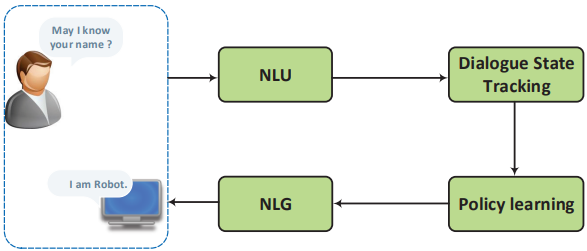
\includegraphics[scale=0.7]{traditional-pipeline}
    \caption{Pipeline general pentru sisteme orientate pe task-uri \cite{chen_liu_yin_tang_dialogue_2017}}
\end{figure}

În plus, există încă multe provocări legate de securitate și confidențialitate care trebuie abordate înainte ca chatbotii să fie adoptați pe scară largă în industria bancară. Acestea includ protejarea datelor personale și financiare ale utilizatorilor și asigurarea că chatbotii nu pot fi utilizați pentru activități frauduloase.

În concluzie, în timp ce adoptarea chatbotilor în sistemul bancar a făcut progrese remarcabile în ultimii ani, există încă multe oportunități de cercetare și dezvoltare în acest domeniu. Pe măsură ce tehnologia continuă să avanseze, este de așteptat ca chatbotii să devină un element tot mai integral al serviciilor bancare.

\section{Obiectivele lucrării în context}

Obiectivul principal al acestei lucrări este de a investiga posibilitățile pe care tehnologia chatbot și serviciile cloud le oferă în contextul sistemului bancar. În particular, accentul este pus pe implementarea unui model de chatbot bazat pe platforma DialogFlow, cu suport pentru limbajul de programare C++. C++ este un limbaj de programare popular, cunoscut pentru eficiența și puterea sa, fiind astfel un candidat potrivit pentru dezvoltarea unui chatbot robust și eficient.

În actualul stadiu de dezvoltare a tehnologiei chatbot, această lucrare vizează să contribuie la progresul subdomeniului, prin oferirea unei viziuni detaliate asupra procesului de implementare a unui chatbot în serviciile bancare, lucrarea speră să aducă o valoare semnificativă domeniului.

În plus, lucrarea explorează și potențialele căi de îmbunătățire și adaptare a chatbotilor. O astfel de direcție ar putea fi folosirea de tehnologii avansate de AI, cum ar fi învățarea profundă, pentru a dezvolta chatboti care pot învăța și se pot adapta la comportamentul și preferințele individuale ale utilizatorilor. Prin urmare, acest studiu își propune să deschidă calea către o utilizare mai extinsă și mai eficientă a tehnologiei chatbot în industria bancară.

Pe de altă parte, această lucrare se concentrează și asupra cloud computing-ului, o tehnologie care a revoluționat modul în care datele și serviciile sunt gestionate. Cu ajutorul cloud computing-ului, chatbotii pot fi ușor scalabili, ceea ce înseamnă că pot servi un număr mare de utilizatori simultan, fără a compromite performanța. În plus, cloud computing-ul facilitează actualizările și îmbunătățirile continuu, fără întreruperi majore ale serviciului \cite{mell_grance2011}.

În concluzie, această lucrare are ca scop principal să demonstreze cum tehnologiile moderne, precum chatbotii și cloud computing-ul, pot transforma modul în care băncile interacționează cu clienții lor. Se urmărește evidențierea beneficiilor potențiale ale utilizării agenților conversaționali pentru optimizarea proceselor și serviciilor bancare, în speranța de a stimula o adoptare mai largă a acestor tehnologii în industria bancară.
\chapter{Decizii arhitecturale}

\section{Ecosistemul Google Cloud}

\subsection{Alegerea platformei agentului}

Comparând Dialogflow cu alte servicii de agenți conversaționali, există mai multe caracteristici care îl diferențiază și îl recomandă pentru utilizarea în sectorul bancar.

Dialogflow, deținut de Google, este o platformă avansată pentru dezvoltarea de aplicații de conversație, care folosește tehnologia AI pentru a interpreta intențiile și contextul utilizatorului \cite{google_dialogflow}. Aceasta oferă o gamă largă de funcționalități, inclusiv integrarea cu diverse platforme de mesagerie, asistenți virtuali și alte servicii Google, cum ar fi Google Cloud Functions.

La rândul lor, serviciile alternative, cum ar fi IBM Watson, Amazon Lex și Microsoft Luis, prezintă și ele avantaje. IBM Watson se remarcă prin puterea sa de a învăța în mod continuu și de a se adapta la diverse contexte de utilizare \cite{ibm_watson}. Amazon Lex beneficiază de integrarea nativă cu ecosistemul Amazon Web Services (AWS), oferind posibilități extinse de dezvoltare și scalare \cite{amazon_lex}. În cele din urmă, Microsoft Luis are avantajul integrării strânse cu suita de produse Microsoft, care includ Office 365 și Azure \cite{microsoft_luis}.

Cu toate acestea, Dialogflow se distinge prin mai multe aspecte-cheie. În primul rând, Dialogflow este foarte flexibil, permițând dezvoltatorilor să creeze experiențe de conversație personalizate pentru diferite platforme și canale de comunicare. Acesta poate fi integrat cu o multitudine de servicii, de la Google Assistant și Amazon Alexa, până la Facebook Messenger și Slack.

În al doilea rând, Dialogflow folosește servicii integrate în ecosistemul Google Cloud. Astfel, permite dezvoltatorilor să creeze, să testeze și să implementeze chatboti direct în cloud, profitând de avantajele acestuia.

Aici intervine Google Cloud Functions \cite{google_cloud_functions}, un serviciu de calcul care permite dezvoltatorilor să execute cod ca răspuns la evenimente specifice, fără a fi nevoie să administreze o infrastructură de server. Acest serviciu poate fi utilizat în tandem cu Dialogflow pentru a crea funcții de backend pentru chatbot, cum ar fi procesarea cererilor utilizatorului, integrarea cu alte sisteme sau baze de date, sau gestionarea autentificării și a securității.

Google Cloud Functions se integrează perfect cu Google Source Repositories \cite{google_source_repositories}, un serviciu de găzduire de cod sursă care oferă un loc sigur și scalabil pentru a stoca și a gestiona codul. Acest lucru permite dezvoltatorilor să colaboreze eficient la proiecte, să gestioneze versiunile de cod și să implementeze automat codul în Cloud Functions.

În final, Google Cloud Storage oferă un serviciu de stocare de obiecte scalabil și durabil, care poate fi utilizat pentru a stoca și a servi datele utilizate de chatbot, cum ar fi înregistrări de conversații, profile de utilizator, sau alte date de context \cite{google_cloud_storage}.

\begin{figure}[h]
    \centering
    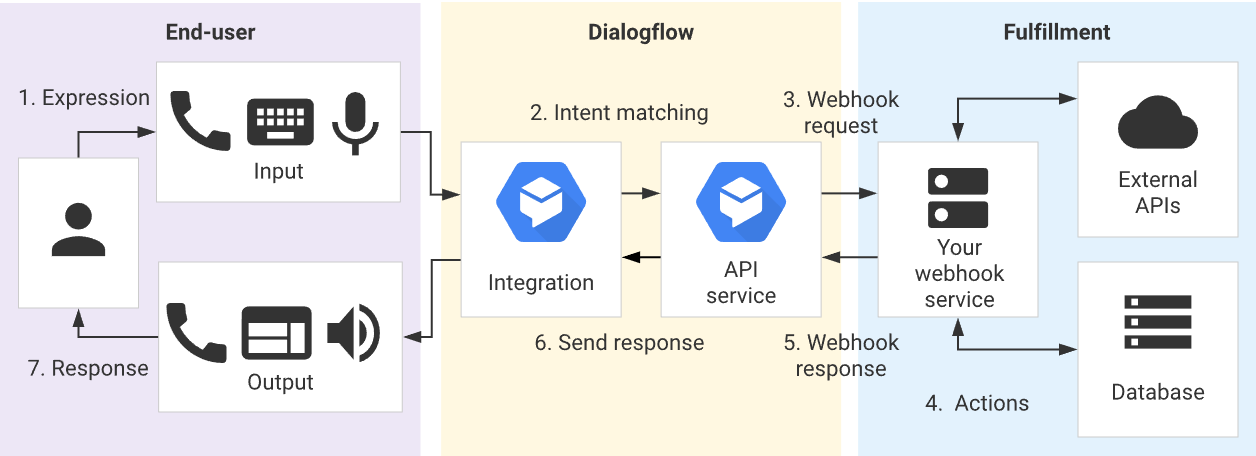
\includegraphics[width=1.0\textwidth]{fulfillment-flow}
    \caption{Flow-ul intern al Dialogflow \cite{google_dialogflow}}
\end{figure}

În ansamblu, alegerea Dialogflow, împreună cu Google Cloud Functions, Google Source Repositories și Google Cloud Storage, oferă o soluție robustă și flexibilă pentru dezvoltarea de chatboti în sectorul bancar. Prin folosirea acestor tehnologii, băncile pot crea experiențe de conversație personalizate, eficiente și securizate pentru clienții lor.

\subsection{Cum funcționează ecosistemul}

Dialogflow folosește input-ul trimis de către Dialogflow API C++ Client \cite{dialogflow_client_library}, acesta fiind parsat și trecut prin verificarea lor internă cu intențiile create în prealabil\footnote{O intenție reprezintă un anumit rezultat pe care doriți să îl obțineți de la interacțiunea utilizatorului. De exemplu, o intenție poate fi „programare întâlnire” sau „informații despre cont”.}. În funcție de cum este creat intent-ul și scopul său, pot exista parametrii scoși sub formă de entități\footnote{Entitățile sunt concepte valoroase care pot fi extrase din declarațiile utilizatorilor. De exemplu, în declarația „Doresc să programez o întâlnire pentru marți”, „marți” este o entitate de tip „dată”.} din textul primit (sau este un intent default, cu rol de legătură între altele cu functionalități).

\begin{figure}[h]
    \centering
    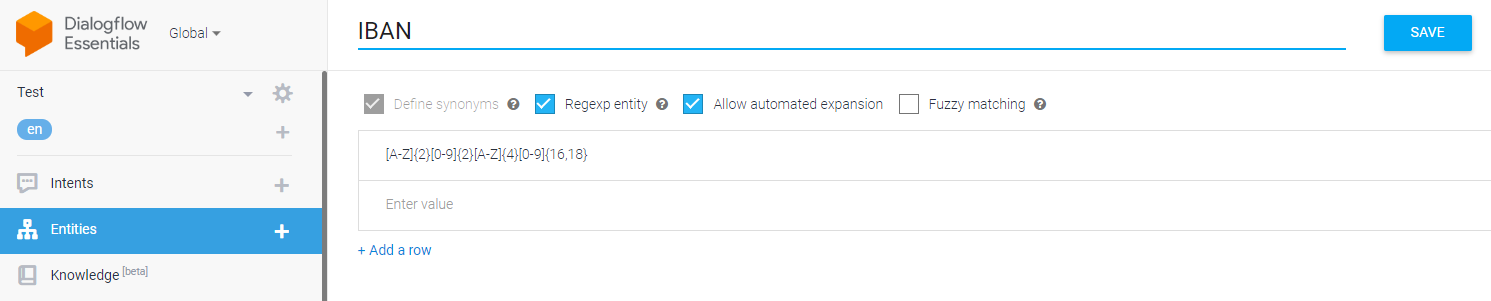
\includegraphics[width=1.0\textwidth]{entitati}
    \caption{Reprezentarea unei entități pentru IBAN folosind un regex}
    \label{fig:entitati}
\end{figure}

În DialogFlow, o "intenție" reprezintă un anumit rezultat pe care îl doriți de la o interacțiune cu utilizatorul. Atunci când un utilizator trimite un input (cum ar fi o întrebare sau o comandă), DialogFlow potrivește inputul cu cea mai bună intenție pe baza a ceea ce ați setat în agentul dvs. În cadrul unei intenții, există mai multe câmpuri și concepte cheie care sunt utilizate pentru a defini și a rafina comportamentul intenției.

\textbf{Contextele} permit agentului DialogFlow să înțeleagă starea conversației și să răspundă în mod corespunzător. Există două tipuri de contexte: contexte de intrare și contexte de ieșire. Contextele de intrare sunt cele pe care agentul le caută înainte de a potrivi o intenție, în timp ce contextele de ieșire sunt stabilite după ce o intenție este potrivită.

\textbf{Exemple de declarații ale utilizatorului} sunt exemple de ceea ce utilizatorul ar putea spune pentru a declanșa această intenție (vezi Figura \ref{fig:training-phrases}). Sistemul utilizează aceste exemple pentru a învăța modelul de limbaj pentru a recunoaște aceeași intenție din declarații diferite.

\begin{figure}[H]
    \centering
    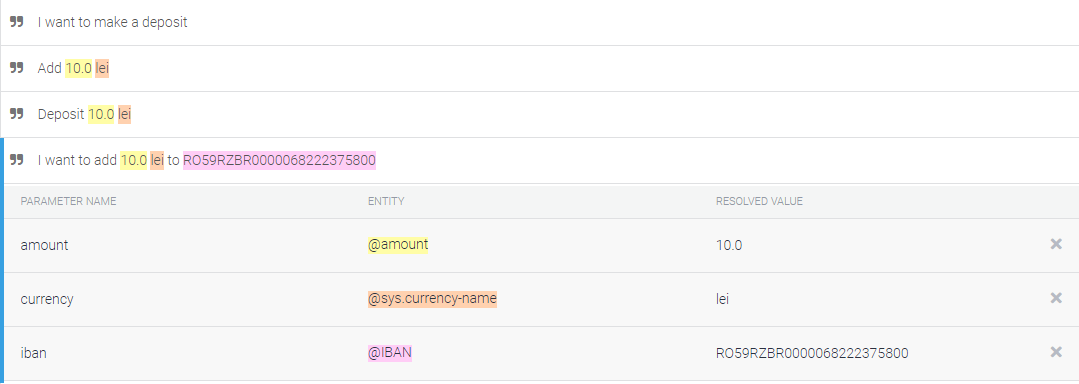
\includegraphics[width=1.0\textwidth]{training-phrases}
    \caption{Frazele de antrenament ale botului}
    \label{fig:training-phrases}
\end{figure}

\textbf{Răspunsurile} reprezintă modul de interacționare hard-codată a agentului cu inputul clientului. Astfel, un răspuns toate fi considerat fie final de conversație, fie poate avea un răspuns default, folosind funcționalitatea webhook-ului ulterior.

\begin{figure}[H]
    \centering
    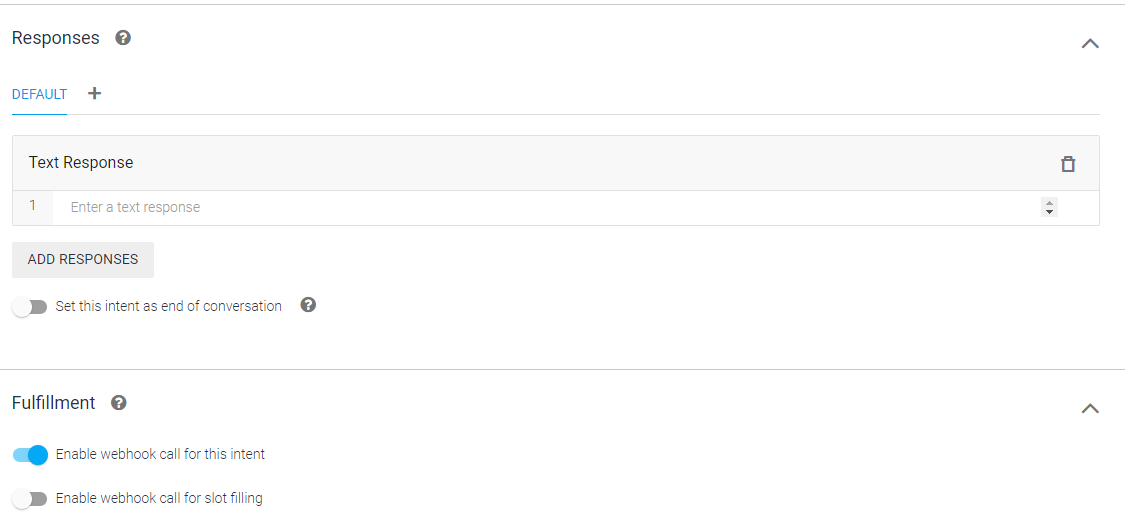
\includegraphics[width=1.0\textwidth]{fulfillment}
    \caption{Selectarea fulfillment-ului}
    \label{fig:fulfillment}
\end{figure}

În cadrul platformei există niște entități predefinite \cite{system-entities} pentru a ușura munca utilizatorului atunci când vine vorba de extragere de parametrii, dar funcționalitatea puternică al acestei opțiuni este extragerea parametrizată a informațiilor. Dupa cum putea vedea in Figura \ref{fig:actiune-parametrii}, acțiunea propriu-zisă oferă flexibilitate atât la prezența parametrului (daca acesta se poate scoate din text), cât și la un text default dacă acesta nu a fost găsit. Coloana \emph{value} reprezintă numele variabilei care este trimisă către metoda din Google Cloud Function, prin webhook-ul definit în tabul de \emph{fulfillment}.

\begin{figure}[h]
    \centering
    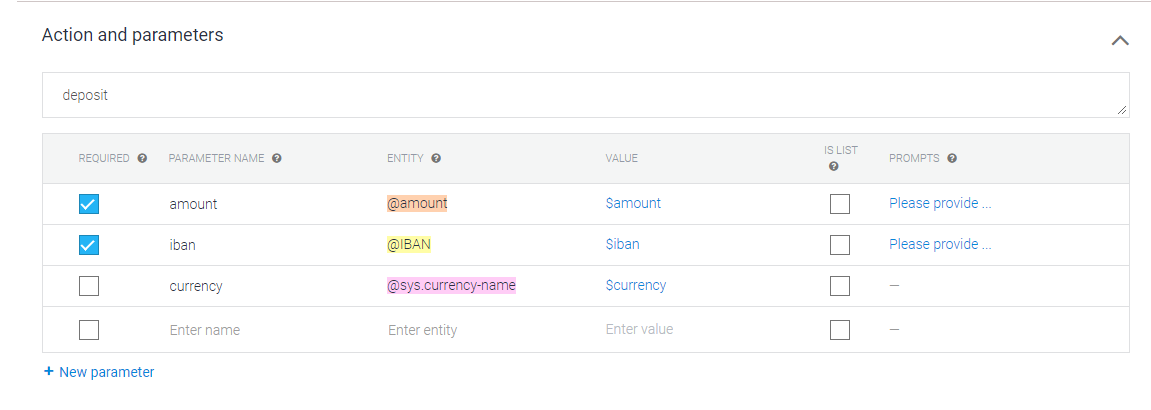
\includegraphics[width=1.0\textwidth]{actiune-parametrii}
    \caption{Extragerea de paramertii din inputul clientului}
    \label{fig:actiune-parametrii}
\end{figure}

În tab-ul de fulfillment putem găsi modul de procesare al informației extrase de către agent. În cazul de față, am folosit un webhook extern, care folosește integrarea cu Google Cloud Function. Astfel, parametrii scoși vor fi trimiși sub forma unui request către acel URL. Detaliile acelui request se află în Figura \ref{fig:exemplu-request}.

\begin{figure}[h]
    \centering
    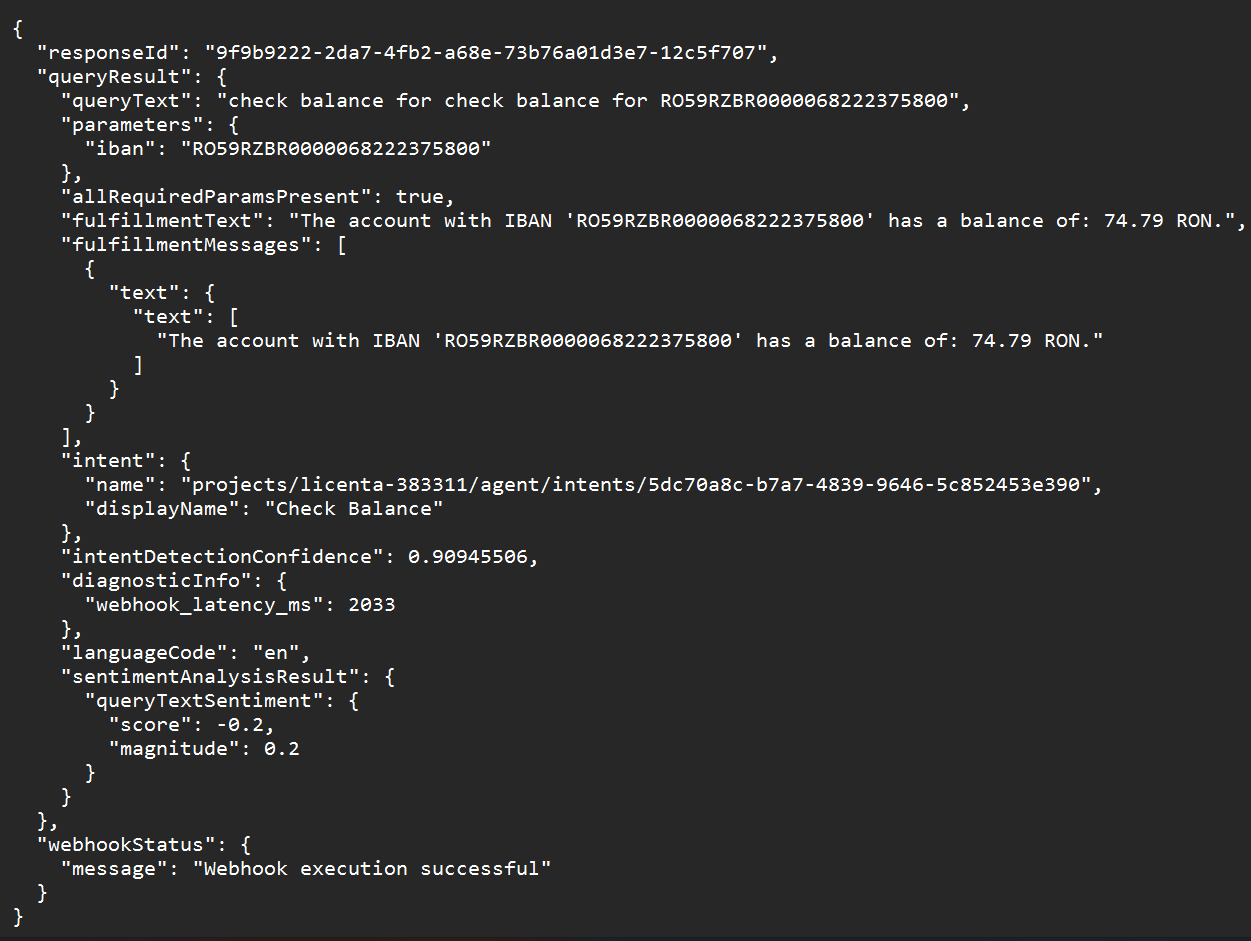
\includegraphics[width=1.0\textwidth]{exemplu-request}
    \caption{Exemplu de request trimis către Google Cloud Function}
    \label{fig:exemplu-request}
\end{figure}

Explicațiile parametrului pentru o mai bună înțelegere a modului de transmitere a informației între seriviciile Google Cloud Platform.

\begin{enumerate}
    \item responseId: acesta este un identificator unic pentru fiecare interacțiune cu DialogFlow.

    \item queryResult: aceasta este secțiunea care conține majoritatea informațiilor legate de interacțiunea cu utilizatorul.
    
    \subitem queryText: aceasta este întrebarea sau afirmația pe care utilizatorul a transmis-o.
    
    \subitem parameters: acestea sunt parametrii extrasi din întrebarea utilizatorului. În acest caz, "iban" este un parametru și valoarea sa este "RO59RZBR0000068222375800".
    
    \subitem allRequiredParamsPresent: acest câmp indică dacă toți parametrii necesari pentru intenție sunt prezenți. În acest caz, este adevărat, ceea ce înseamnă că toți parametrii necesari sunt prezenți.
    
    \subitem fulfillmentText: acesta este textul care va fi returnat utilizatorului ca răspuns la întrebarea sa.
    
    \subitem fulfillmentMessages: aceasta este o listă de mesaje care vor fi trimise înapoi utilizatorului. În acest caz, este doar un mesaj, care este același cu fulfillmentText.
    
    \subitem intent: aceasta este intenția care a fost potrivită pentru întrebarea utilizatorului.
    
    \subitem intentDetectionConfidence: acesta este gradul de încredere cu care DialogFlow a potrivit intenția. În acest caz, este de aproximativ 93%.
    
    \subitem diagnosticInfo: acestea sunt informații suplimentare privind interacțiunea. În acest caz, indică timpul de latență pentru webhook.
    
    \subitem languageCode: acesta este codul de limbă al interogării utilizatorului.
    
    \subitem sentimentAnalysisResult: aceasta este analiza sentimentului textului interogării. Scorul indică sentimentul general (pozitiv sau negativ), iar magnitudinea indică intensitatea sentimentului.
    
    \item webhookStatus: acesta este statusul execuției webhook-ului, care în acest caz a fost reușită.
\end{enumerate}

Tabul de "Validation" din DialogFlow ES are de-a face cu revizuirea și aprobarea sau respingerea propunerilor pe care DialogFlow le face pentru îmbunătățirea modelului asistentului virtual. Acesta este un element al învățării automate interactive, unde sistemul învață din feedbackul dat de utilizator.

După ce asistentul virtual a fost folosit o vreme, va începe să învețe din interacțiunile cu utilizatorii și va încerca să îmbunătățească precizia detecției intențiilor și a entităților. Acest lucru este realizat prin generarea de "sugestii" pe baza interacțiunilor anterioare. Aceste sugestii apar în tabul "Validation".

Fiecare sugestie conține următoarele elemente:

Training phrase - Este textul interacțiunii dintre utilizator și asistentul virtual.

Intent - Este numele intenției pe care DialogFlow o propune pentru fraza de instruire. Acesta poate fi o intenție existentă sau o nouă intenție sugerată de DialogFlow.

Action - Este un câmp opțional, care permite asocierea unei acțiuni cu o intenție. DialogFlow poate sugera o acțiune pe baza contextului frazei de instruire.

Entities - Sunt entitățile pe care DialogFlow le propune pentru a fi asociate cu fraza de instruire.

Fiecare sugestie poate fi aprobată sau respinsă, în funcție de dorință (vezi Figura \ref{fig:validation}). Dacă sugestia este aprobată, DialogFlow va actualiza modelul asistentului virtual pentru a include informațiile din sugestie, îmbunătățind astfel precizia detecției de intenții și entități în interacțiunile viitoare. Dacă sugestia este respinsă, DialogFlow nu va face nicio modificare.

\begin{figure}[h]
    \centering
    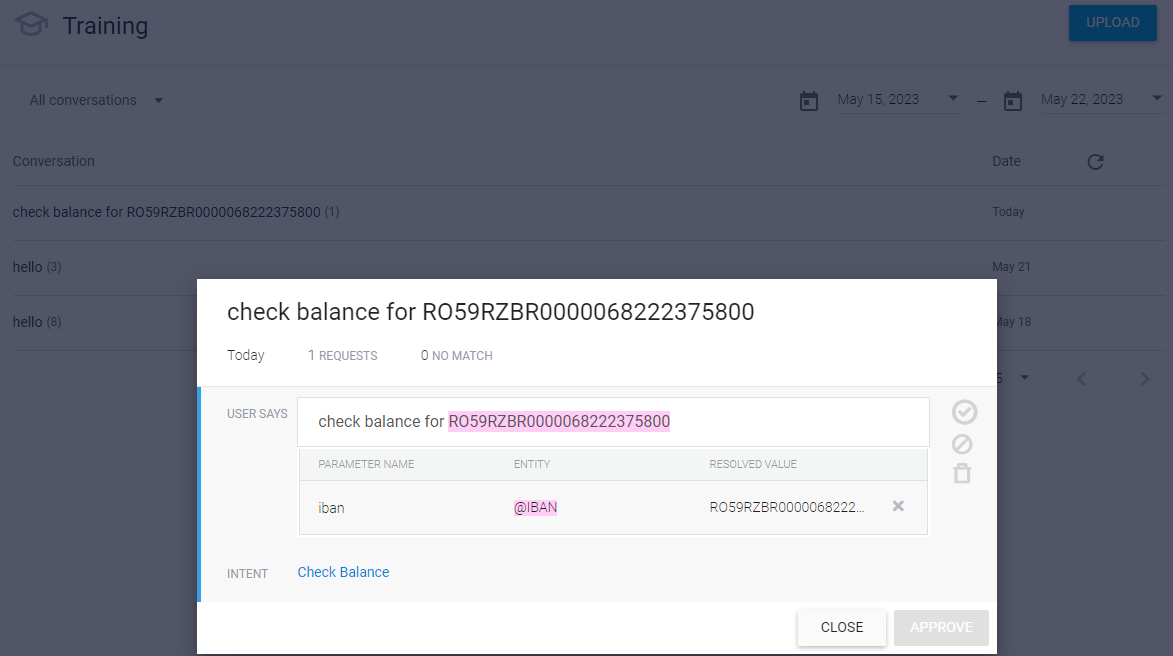
\includegraphics[width=1.0\textwidth]{validation}
    \caption{Validarea rezultatului agentului}
    \label{fig:validation}
\end{figure}

\section{Alegerea utilitarului}

Biblioteca Portable Components (POCO) este un set popular de biblioteci open-source pentru dezvoltarea de software în C++. Se evidențiază printr-o gamă largă de facilități care îi permit să fie o soluție potrivită pentru dezvoltarea unei aplicații web. Înainte de a trece la detaliile bibliotecii POCO, este esențial să se înțeleagă contextul general al instrumentelor și bibliotecilor disponibile pentru dezvoltarea aplicațiilor web în C++.

Din punct de vedere istoric, dezvoltarea aplicațiilor web în C++ a fost deseori privită ca un proces complex, în mare parte din cauza faptului că limbajul C++ este orientat spre dezvoltarea software de nivel înalt, cu un control detaliat asupra resurselor hardware, precum și a complexității implicite a acestui limbaj. Cu toate acestea, cu ajutorul unor instrumente precum bibliotecile POCO \cite{poco-docs}, Boost \cite{boost-docs}, Wt \cite{wt-docs} și CPPCMS \cite{cppcms-docs}, dezvoltarea aplicațiilor web în C++ a devenit mult mai ușoară și mai eficientă.

\subsection{POCO: avantaje și caracteristici}

POCO se distinge prin designul său robust și portabil, care permite dezvoltatorilor să creeze software eficient și de înaltă performanță, care poate fi portat cu ușurință pe diferite platforme și sisteme de operare. Bibliotecile POCO au fost concepute pentru a fi ușor de înțeles și de utilizat, fără a impune niciun model de programare specific. Acest lucru le face flexibile și adaptabile, încurajând dezvoltarea rapidă și agile.

În contextul dezvoltării aplicațiilor web, biblioteca POCO oferă numeroase facilități, inclusiv suport pentru HTTP, FTP, sendmail, URI, cookie-uri, HTML formular, și altele. Acesta include, de asemenea, un framework pentru servere web, care permite dezvoltarea serverelor web multithreaded și sigure. De asemenea, biblioteca NetSSL furnizează suport pentru comunicațiile securizate SSL/TLS, care sunt esențiale pentru orice aplicație web modernă.

\subsection{POCO în comparație cu alte biblioteci C++}

Să comparam acum POCO cu alte biblioteci C++ populare pentru dezvoltarea aplicațiilor web: Boost, Wt și CPPCMS.

Boost este o colecție vastă de biblioteci C++, care oferă o gamă largă de facilități. Cu toate acestea, Boost nu este specializat în dezvoltarea aplicațiilor web și nu include suport direct pentru HTTP sau alte protocoale web specifice. Prin urmare, dezvoltarea unei aplicații web cu Boost ar necesita o cantitate semnificativă de cod adițional sau utilizarea altor biblioteci pentru a acoperi aceste funcționalități.

Wt este o bibliotecă C++ pentru dezvoltarea aplicațiilor web care utilizează un model de programare similar cu cel al Qt. Deși Wt este puternic și flexibil, are un model de programare mai complex decât POCO și poate fi mai dificil de învățat și de utilizat, în special pentru cei care nu sunt familiarizați cu Qt.

CPPCMS este un framework specializat pentru dezvoltarea aplicațiilor web în C++. Deși CPPCMS include o serie de facilități puternice pentru dezvoltarea aplicațiilor web, el impune un anumit model de programare, care poate fi mai restrictiv decât abordarea mai flexibilă a POCO.

În concluzie, POCO oferă un echilibru excelent între ușurința de utilizare, flexibilitate, portabilitate și performanță, ceea ce o face o alegere bună pentru dezvoltarea aplicațiilor web în C++. Cu toate acestea, alegerea finală ar trebui să depindă de cerințele specifice ale proiectului, de preferințele dezvoltatorului și de alte considerații.
\chapter{Setup și compilare}

\section{Instalarea bibliotecilor}
Utilizatorul trebuie să aibă o cheie de acces pentru un cont de serviciu pe platforma Google Cloud pentru a accesa API-ul Dialogflow ES. Această cheie trebuie plasată sub directorul \emph{res} \cite{keys-create-delete}.

Această cheie va fi setată ca variabilă de mediu \texttt{GOOGLE\_APPLICATION\_CREDENTIALS}, care va funcționa ca un sistem de autentificare pentru platformă.

În directorul rădăcină al proiectului, se află un script Bash numit \texttt{getting\_started.sh} (Notă: dacă scriptul nu poate fi rulat pe o platformă Unix, se recomandă verificarea formatului greșit al sfârșitului de linie prin executarea comenzii \texttt{dos2unix} pentru script și verificarea din nou). Când este rulat pe o platformă Unix, acesta va instala toate dependențele necesare (vezi \hyperref[first-time-setup]{Configurarea inițială}). După finalizarea scriptului, utilizatorul trebuie să ruleze manual configurarea inițială pentru CLI-ul GC:

\begin{verbatim}
./google-cloud-sdk/install.sh
source ~/.bashrc
./google-cloud-sdk/bin/gcloud init
\end{verbatim}

Notă: Configurarea inițială va dura un timp \textbf{îndelungat} (în special pe mașini mai vechi).

\section{Configurarea inițială}
Fluxul scriptului \texttt{getting\_started.sh} este următorul:

\textbf{Notă importantă}: Trebuie să fie rulat cu opțiunea \texttt{-i} sau \texttt{--install}, iar după finalizarea acestuia, utilizatorul trebuie să ruleze manual configurarea inițială pentru gcloud (vezi pașii de mai sus).

\begin{enumerate}
  \item Configurarea mediului:
    \begin{enumerate}
      \item Submodulele sunt inițializate.
      \item Pe baza diferenței în terminarea greșită a liniei, atât scriptul \texttt{build.sh}, cât și executabilul \texttt{sass} vor fi convertite la formatul Unix-like.
      \item Se instalează \texttt{doxygen} și dependența sa \texttt{graphviz}.
    \end{enumerate}
  \item Revenirea la versiunile dorite ale bibliotecilor:
    \begin{enumerate}
      \item Se utilizează versiunea \texttt{POCO v1.12.4}.
      \item Se utilizează versiunea \texttt{VCPKG v2023.04.15 Release}.
      \item Se utilizează versiunea \texttt{GCP v2.9.1}.
    \end{enumerate}
  \item Configurarea POCO \cite{poco}:
    \begin{enumerate}
      \item Se instalează dependențele (\texttt{openssl, libssl-dev, git, g++, make, cmake}).
      \item Se configurează fișierul \texttt{CMakeLists.txt}.
      \item Se construiește fișierul de configurare.
      \item Se instalează biblioteca.
    \end{enumerate}
  \item Configurarea npm:
    \begin{enumerate}
      \item Se instalează \texttt{npm} prin intermediul gestionarului de pachete implicit.
    \end{enumerate}
  \item Configurarea Google Cloud CLI \cite{gcloud-cli}:
    \begin{enumerate}
      \item Se descarcă arhiva care conține codul sursă.
      \item Se extrage arhiva.
    \end{enumerate}
  \item Configurarea Sass:
    \begin{enumerate}
      \item Se creează un link simbolic (\texttt{symlink}) și se forțează crearea acestuia, chiar dacă există, către executabilul furnizat (vezi directorul \texttt{libs/sass}).
    \end{enumerate}
  \item Configurarea VCPKG \cite{vcpkg}:
    \begin{enumerate}
      \item Se instalează dependențele (\texttt{curl, zip, unzip, tar}).
      \item Se configurează managerul vcpkg pentru prima dată prin intermediul scriptului de pornire (\texttt{libs/vcpkg/bootstrap-vcpkg.sh}).
    \end{enumerate}
  \item Configurarea Google Cloud Platform \cite{dialogflow_quickstart}:
    \begin{enumerate}
      \item Se instalează modulele reale pe care le vom utiliza în proiect (\texttt{core} și \texttt{dialogflow-es}) prin intermediul vcpkg.
    \end{enumerate}
\end{enumerate}

\section{Cum se construiește}
Din directorul rădăcină al proiectului, putem utiliza scriptul \texttt{build.sh} pentru a construi și rula aplicația. În mod implicit, serverul va utiliza portul \textbf{9090}, dar acesta poate fi modificat din fișierul \texttt{constants.h} (vezi \texttt{globals::serverPort}).

Există câteva opțiuni care pot fi utilizate cu scriptul:
\begin{itemize}
  \item \texttt{-b} sau \texttt{--build} => compilează și rulează proiectul
  \item \texttt{-bscss} sau \texttt{--build-scss} => compilează doar fișierele SCSS pentru a actualiza aspectul HTML-ului
  \item \texttt{-docs} sau \texttt{--generate-docs} => generează documentația tehnică utilizând Doxygen
  \item \texttt{-c} sau \texttt{--clean} => curăță proiectul
  \item \texttt{-v} sau \texttt{--verbose} => opțional, afișează mai multe informații în consolă
  \item \texttt{-h} sau \texttt{--help} => afișează această informație de ajutor
\end{itemize}

Notă: Nu se recomandă rularea opțiunii \texttt{-c} împreună cu alte opțiuni, deoarece curățarea trebuie să fie un proces singular.
\chapter{Detalierea implementării}

\section{Script-uri auxiliare}

Ambele scripturi folosesc același cod pentru prelucrarea inputului utilizatorului și tratarea erorilor.

Acestea sunt procesate de funcția \texttt{func\_read\_cli\_options} și sunt verificate cu lista implicită (care diferă în mare parte pentru ambele scripturi, deoarece au roluri distincte, dar opțiunile \texttt{-v} și \texttt{-h} sunt comune, deoarece au o utilitate comună).

\begin{itemize}
  \item Flaguri comune:
    \begin{itemize}
      \item Flagul \texttt{verbose} permite scripturilor să afișeze mai multe informații (atât de la ele, cât și din jurnalele aplicației) în consolă. Această opțiune va seta variabila globală \texttt{VERBOSE} la true.
      \item Flagul \texttt{help} va afișa doar informațiile de ajutor.
    \end{itemize}
  \item Flagurile specifice pentru \texttt{getting\_started.sh}:
    \begin{itemize}
      \item Flagul \texttt{install} instalează și configurează toate dependențele pentru proiect.
    \end{itemize}
  \item Flagurile specifice pentru \texttt{build.sh}:
    \begin{itemize}
      \item Flagul \texttt{build} va compila și executa proiectul.
      \item Flagul \texttt{build-scss} va compila doar fișierele SCSS pentru a actualiza aspectul HTML-ului.
      \item Flagul \texttt{generate-docs} va genera documentația tehnică utilizând Doxygen.
      \item Flagul \texttt{clean} va curăța proiectul de fișiere temporare, jurnale, executabile, fișiere binare, etc.
    \end{itemize}
\end{itemize}

Dacă Flagul există în lista dorită, variabila \texttt{COMMAND} stochează acțiunea dorită și apoi este pasată funcției \texttt{execute}.

Funcția \texttt{execute} va apela apoi metoda corespunzătoare funcționalității dorite. Acest nivel de abstractizare permite concatenarea mai multor comenzi sub același nume, dacă este necesar.

Notă: Din acest moment înainte, se va analiza fiecare script în mod individual, deoarece au metode diferite pentru cazurile lor de utilizare diferite.

Iată codul LaTeX actualizat, utilizând listele pentru enumerare:

\subsection{Getting Started}
Pentru \texttt{getting\_started.sh}:

\begin{itemize}
    \item Metoda \texttt{execute} poate apela doar funcția \texttt{install}. Această metodă va parcurge o listă de comenzi și va instala dependențele necesare (vezi \hyperref[first-time-setup]{Configurarea inițială}).
\end{itemize}

\subsection{Build}
Pentru \texttt{build.sh}:

\begin{itemize}
    \item Metoda \texttt{execute} poate apela una dintre următoarele funcții:
    \begin{itemize}
        \item Funcția \texttt{compile\_sass} va itera peste toate fișierele SCSS din subfolderul \texttt{res/scss} și le va compila, generând fișierele CSS dorite în subfolderul \texttt{res/css}. Aceste fișiere nu vor conține hărți CSS generate automat, deoarece nu există mult CSS pentru început și nu este necesară crearea unei logici suplimentare pentru ca serverul să gestioneze aceste solicitări.
        \item Funcția \texttt{generate\_docs} va genera documentația tehnică. În fișierul Doxyfile, următoarele taguri au fost modificate:
        \begin{itemize}
            \item \texttt{PROJECT\_NAME = "Licență"}
            \item \texttt{PROJECT\_BRIEF = "O aplicație bancară C++ care utilizează Dialogflow ES de pe Google Cloud Platform pentru interacțiuni uman-bot într-un context bancar."}
            \item \texttt{OUTPUT\_DIRECTORY = "./res/docs"}
            \item \texttt{FULL\_PATH\_NAMES = NO}
            \item \texttt{BUILTIN\_STL\_SUPPORT = YES}
            \item \texttt{EXTRACT\_ALL = YES}
            \item \texttt{EXTRACT\_PRIVATE = YES}
            \item \texttt{EXTRACT\_STATIC = YES}
            \item \texttt{INPUT = ./res}
            \item \texttt{RECURSIVE = YES}
            \item \texttt{HTML\_OUTPUT = .}
            \item \texttt{DISABLE\_INDEX = YES}
            \item \texttt{GENERATE\_TREEVIEW = YES}
            \item \texttt{GENERATE\_LATEX = NO}
            \item \texttt{CALL\_GRAPH = YES}
            \item \texttt{CALLER\_GRAPH = YES}
            \item \texttt{ALPHABETICAL\_INDEX = NO}
        \end{itemize}
        \item Funcția \texttt{build} este o metodă de nivel superior care are ca scop construirea și rularea executabilului final. Executabilul se numește \texttt{licenta\_EXECUTABLE} și poate fi găsit în directorul rădăcină al proiectului. Acesta poate fi rulat cu două indicatoare: \texttt{DISABLE\_DEBUG} sau \texttt{ENABLE\_DEBUG}. Aceste indicatoare depind de valoarea variabilei globale \texttt{VERBOSE}. Dacă este \texttt{true}, sistemul de jurnalizare al proiectului (\texttt{MyLogger} - un wrapper peste clasa \texttt{Poco's Logger}) va crea un canal \texttt{Poco::ConsoleChannel}, care va fi furnizat unui canal \texttt{Poco::SplitterChannel}. Astfel, orice jurnal se va genera, va fi afișat și în consolă, pe lângă folderul \texttt{logs}.
        \item \begin{enumerate}
            \item Funcția \texttt{build} este o metodă de nivel superior care are ca scop construirea și rularea executabilului final. Executabilul se numește \texttt{licenta\_EXECUTABLE} și poate fi găsit în directorul rădăcină al proiectului. Acesta poate fi rulat cu două indicatoare: \texttt{DISABLE\_DEBUG} sau \texttt{ENABLE\_DEBUG}. Aceste indicatoare depind de valoarea variabilei globale \texttt{VERBOSE}. Dacă este \texttt{true}, sistemul de jurnalizare al proiectului (\texttt{MyLogger} - un wrapper peste clasa \texttt{Poco's Logger}) va crea un canal \texttt{Poco::ConsoleChannel}, care va fi furnizat unui canal \texttt{Poco::SplitterChannel}. Astfel, orice jurnal se va genera, va fi afișat și în consolă, pe lângă folderul \texttt{logs}.
            \item Se apelează funcția \texttt{compile\_sass}. Consultați mai sus pentru mai multe explicații.
            \item Funcția \texttt{compile\_cpp} configurează mai întâi fișierul \texttt{CMakeLists.txt} și trece variabila \texttt{CMAKE\_TOOLCHAIN\_FILE} la CMake-ul de pe Google Cloud Platform. Deoarece aceasta nu este utilizată direct în acest CMake, vom adăuga și indicativul \texttt{--no-warn-unused-cli} pentru a suprima avertismentul referitor la această variabilă. Dacă configurarea reușește, se va efectua construirea efectivă a proiectului.
            \item Funcția \texttt{configure\_gcp} va exporta variabila \texttt{GOOGLE\_APPLICATION\_CREDENTIALS}, astfel încât să fie vizibilă pentru fiecare proces și subproces care pornește din script.
        \end{enumerate}
    \end{itemize}
\end{itemize}

Proiectul CMake utilizează standardul \texttt{C++17}, iar executabilul este generat în directorul rădăcină al proiectului. Bibliotecile utilizate pentru legare sunt \texttt{Poco::Foundation Poco::Net Poco::Util google-cloud-cpp::dialogflow\_es}.

\section{Logica agentului}

Codul poate fi găsit în \textbf{./cloud} și constă într-un scrip JavaScript utilizat în contextul unui serviciu de îndeplinire a cerințelor (fulfillment) pentru Dialogflow, un serviciu de înțelegere a limbajului natural și de gestionare a conversațiilor dezvoltat de Google. Acest script gestionează cererile primite de la Dialogflow și furnizează răspunsurile corespunzătoare. De asemenea acesta este rulat prin Google Cloud Function, codul fiind luat din serviciul Google Source Repository.

La nivel top-level, se regăsesc următoarele funcționalități:

\begin{enumerate}
    \item Se importă modulele necesare: `firebase-functions`, `dialogflow-fulfillment`, `google-cloud/storage` și `axios`. Aceste module facilitează comunicarea cu Dialogflow, gestionarea stocării și efectuarea de cereri HTTP.

    \item Se definește funcția `dialogflowFirebaseFulfillment` ca o funcție de tip `functions.https.onRequest`, care va fi apelată în momentul în care se primește o cerere HTTP către URL-ul specificat în configurația Firebase.

    \item În interiorul funcției `dialogflowFirebaseFulfillment`, se inițializează un obiect `WebhookClient` cu request-ul și response-ul primite. Acest obiect facilitează procesarea cererii și furnizarea răspunsului către Dialogflow.

    \item Se definesc funcțiile care vor fi apelate în funcție de intent-ul identificat de Dialogflow. Aceste funcții gestionează diferite scenarii de conversație și furnizează răspunsuri specifice. De exemplu, funcția `welcome` furnizează un mesaj de bun venit, iar funcția `checkBalance` verifică soldul unei anumite conturi bancare. Fiecare funcție primește ca parametru obiectul `agent`, care reprezintă un context de conversație și permite adăugarea de mesaje și interacțiune cu utilizatorul.

    \item În cadrul funcțiilor, se folosește obiectul `agent` pentru a adăuga mesaje de răspuns, a efectua verificări și a interacționa cu sistemul de stocare în cloud folosind modulul `google-cloud/storage`.

    \item Funcția `getConversionRate` este utilizată pentru a obține rata de conversie între două valute folosind un serviciu extern. Această funcție face o cerere HTTP către un API și returnează rata de conversie.

    \item Este creată o instanță a obiectului `WebhookClient` și se apelează funcția `handleRequest` pentru a procesa cererea și a furniza răspunsul corespunzător.

    \item Este definită o hartă de intent-uri (`intentMap`) care asociază funcțiile definite mai sus cu intent-urile specifice. Astfel, în funcția `handleRequest`, se va apela funcția corespunzătoare în funcție de intent-ul identificat de Dialogflow.
\end{enumerate}

Acest script oferă suport pentru diferite funcționalități de gestionare a conversațiilor cu un chatbot, cum ar fi verificarea soldului, transferul de bani între conturi, crearea și ștergerea de conturi bancare. De asemenea, folosește un serviciu extern pentru a obține ratele de conversie valutară. Prin intermediul acestui script, se poate crea un chatbot interactiv și inteligent care să furnizeze răspunsuri personalizate și să interacționeze cu utilizatorii într-un mod natural.

\section{Logica locală}

Arhitectural vorbind, partea din aplicație care se află local reprezinta doar scheletul funcționalității principale, partea importantă fiind mutată în serviciile oferite de Google Cloud Platform.

\begin{figure}[h]
  \centering
  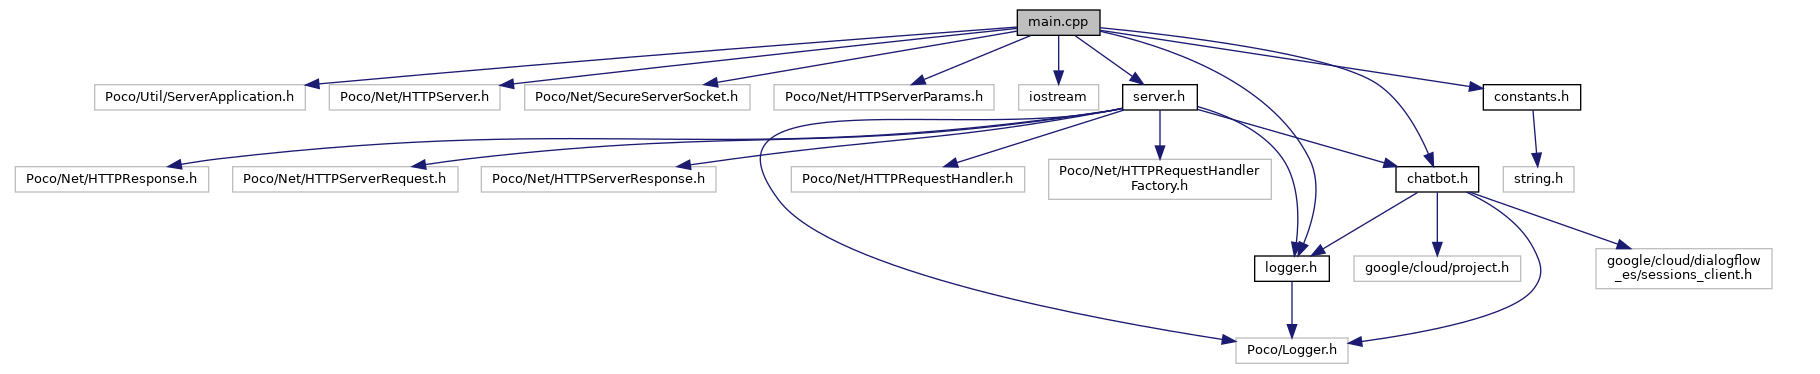
\includegraphics[width=1.0\textwidth]{include-graph}
  \caption{Include graph-ul principal.}
  \label{fig:includeGraph}
\end{figure}

\subsection{Main}

Codul începe prin includerea mai multor fișiere de bibliotecă necesare pentru funcționalitatea serverului. Aceste fișiere de bibliotecă sunt:

\begin{itemize}
  \item Poco/Util/ServerApplication.h: Această bibliotecă conține clasa ServerApplication, care oferă funcționalități pentru implementarea unei aplicații server.
  \item Poco/Net/HTTPServer.h: Această bibliotecă conține clasa HTTPServer, care gestionează cererile HTTP primite de la clienți.
  \item Poco/Net/SecureServerSocket.h: Această bibliotecă conține clasa SecureServerSocket, care permite comunicarea securizată între server și clienți utilizând SSL/TLS.
  \item Poco/Net/HTTPServerParams.h: Această bibliotecă conține clasa HTTPServerParams, care permite configurarea parametrilor serverului HTTP.
\end{itemize}

În plus față de bibliotecile POCO, codul include și alte fișiere specifice aplicației, cum ar fi "server.h", "logger.h", "chatbot.h" și "constants.h". Aceste fișiere conțin declarații și implementări specifice aplicației și sunt utilizate în codul principal pentru a oferi funcționalitatea dorită.

După includerea fișierelor de bibliotecă și a fișierelor specifice aplicației, se utilizează namespace-ul Poco::Util pentru a evita utilizarea repetată a acestuia în cod.

Următoarea parte a codului definește clasa MyServerApp, care este o clasă derivată din ServerApplication. Această clasă acționează ca un wrapper peste clasa ServerApplication și permite rularea aplicației ca un daemon Unix. Aceasta înseamnă că aplicația poate fi rulată în fundal, fără o interfață grafică și fără a bloca consola (vezi Figura \ref{fig:exempluConversatie}).

\begin{figure}[h]
    \centering
    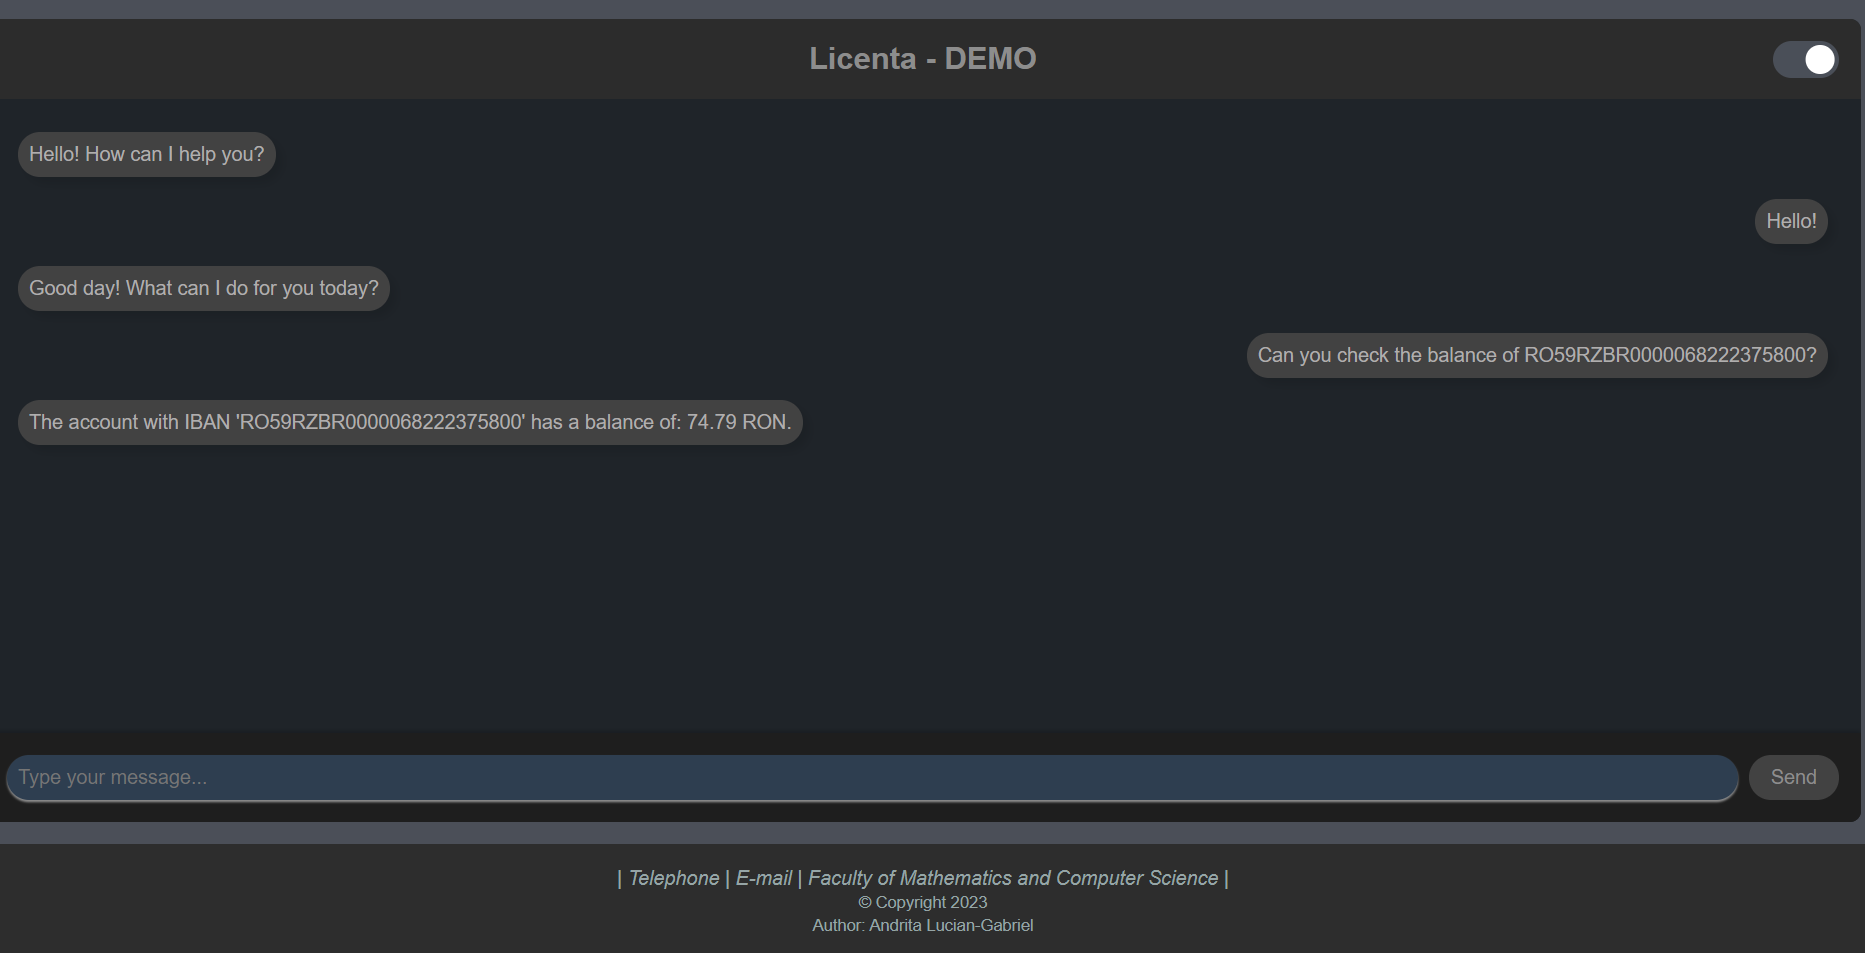
\includegraphics[width=1.0\textwidth]{exemplu-conversatie}
    \caption{Exemplu de conversație.}
    \label{fig:exempluConversatie}
\end{figure}

Clasa MyServerApp conține o metodă main suprascrisă, care implementează funcționalitatea serverului. În această metodă, se configurează parametrii serverului HTTP utilizând clasa HTTPServerParams. Parametrii, cum ar fi numărul maxim de conexiuni acceptate și numărul maxim de thread-uri, sunt setați în acest pas.

Apoi, se creează un obiect de tip HTTPServer utilizând clasa HTTPServer și se specifică un MyRequestHandlerFactory care se ocupă de generarea handler-elor pentru cererile primite de la clienți. De asemenea, se specifică portul serverului utilizând obiectul ServerSocket și se folosesc parametrii configurați anterior pentru a inițializa serverul.

După ce serverul este creat și configurat, acesta este pornit utilizând metoda start a obiectului HTTPServer. În plus, se afișează un mesaj de informare folosind obiectul \textbf{logger} sau prin afișarea directă la consolă.

\subsection{Chatbot}

Clasa Chatbot este responsabilă pentru gestionarea comunicării cu Google Cloud Platform pentru trimiterea și primirea informațiilor. Această clasă este implementată ca un singleton, ceea ce înseamnă că există o singură instanță a acestei clase în întregul program.

Pentru a utiliza funcționalitățile necesare pentru comunicarea cu Google Cloud Platform, avem incluse mai multe fișiere de bibliotecă, cum ar fi "google/cloud/dialogflow\_es/sessions\_client.h", "google/cloud/project.h" și "Poco/Logger.h". Aceste fișiere de bibliotecă conțin clase și funcționalități esențiale pentru interacțiunea cu platforma de cloud.

În cadrul clasei Chatbot, avem o serie de metode și membri de date importante. Pentru a asigura că există o singură instanță a clasei Chatbot, avem metoda statică `getInstance()` care verifică dacă obiectul `agent` a fost deja creat. Dacă da, returnează referința către această instanță existentă, iar dacă nu, creează o nouă instanță și returnează referința către aceasta. Acest mecanism de singleton asigură că avem o singură instanță a clasei Chatbot în întregul program.

O altă metodă importantă este `sendMessage(const std::string\& message)` care primește un mesaj de la client și îl setează ca text de intrare pentru obiectul `request`. Apoi, obiectul `client` trimite informația la Google Cloud Platform și așteaptă un răspuns. Dacă textul de completare din răspuns este gol, un mesaj implicit este stocat în membrul `outputText` al obiectului `agent`. Această metodă asigură trimiterea mesajelor și primirea răspunsurilor în cadrul conversației cu platforma de cloud.

Există și metode pentru setarea și obținerea textului de ieșire al agentului, respectiv `setOutputText(const std::string\& outputParam)` și `getOutputText()`. Aceste metode permit manipularea și accesarea textului de ieșire generat de agentul de chat.

În plus, clasa Chatbot conține și membri de date relevanți pentru funcționarea acesteia. Avem un obiect `logger` de tip Poco::Logger, care este utilizat pentru înregistrarea mesajelor de sistem și este accesibil prin intermediul clasei Logger definită în fișierul "logger.h". De asemenea, avem un obiect `client` de tip dialogflow\_es::SessionsClient care gestionează interacțiunea cu sesiunile de comunicare cu platforma de cloud. Un alt membru important este obiectul `request` de tip v2::DetectIntentRequest care reprezintă cererea de comunicare trimisă la platforma de cloud.

În general, clasa Chatbot oferă o interfață simplificată pentru trimiterea și primirea mesajelor către/de la Google Cloud Platform, facilitând astfel implementarea unui agent de chat funcțional. Această clasă utilizează bibliotecile și funcționalitățile oferite de Google Cloud Platform și POCO pentru a asigura o comunicare eficientă și robustă.

\begin{figure}[h]
  \centering
  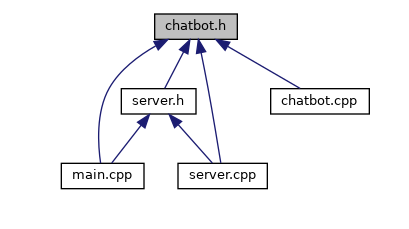
\includegraphics[width=0.8\textwidth]{include-graph-chatbot}
  \caption{Include graph-ul pentru clasa Chatbot.}
  \label{fig:includeGraphChatbot}
\end{figure}

\subsection{Constants}

În codul de mai sus, avem fișierul header "constants.h" care conține câteva constante și un namespace pentru variabilele de configurare utilizate în program.

În interiorul namespace-ului "globals", avem mai multe constante definite:
\begin{enumerate}
    \item "serverPort" reprezintă portul folosit pentru server și are valoarea 9090.
    \item "projectID" reprezintă numele proiectului utilizat pe platforma Google Cloud și are valoarea "licenta-383311".
    \item "sessionID" reprezintă ID-ul sesiunii utilizate pentru client și are valoarea "123456789".
    \item "agentLanguage" reprezintă limba sesiunii și are valoarea "en" (engleză).
\end{enumerate}

Aceste constante sunt folosite în cadrul programului pentru a configura și personaliza diferite aspecte legate de comunicarea cu platforma Google Cloud.

Fișierul header "constants.h" este protejat împotriva includerii multiple în codul sursă utilizând macro-ul de preprocesare "\#ifndef CONSTANTS\_H\_" și "\#endif", ceea ce asigură că fișierul este inclus o singură dată în cadrul unui fișier sursă.

Utilizarea acestor constante și a namespace-ului "globals" asigură o gestionare eficientă a valorilor de configurare în cadrul programului și facilitează modificarea acestora într-un singur loc. Aceasta oferă flexibilitate și ușurință în adaptarea programului la diferite scenarii și cerințe specifice.

\begin{figure}[h]
  \centering
  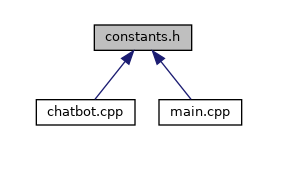
\includegraphics[width=0.6\textwidth]{include-graph-constants}
  \caption{Include graph-ul pentru clasa Constants.}
  \label{fig:includeGraphConstants}
\end{figure}

\subsection{Logger}

Clasa "MyLogger" care este un wrapper singleton peste clasa Poco::Logger. Acesta este un sistem de înregistrare și logging oferit de biblioteca POCO. 

La nivel top-level, clasa "MyLogger" oferă următoarele funcționalități:

\begin{itemize}
    \item Metoda statică "getLogger()" verifică dacă obiectul logger a fost deja creat și returnează o referință către acel obiect. Dacă obiectul nu a fost creat, se va crea un canal pentru fluxul de consolă și un canal pentru fluxul sistemului de fișiere. Se setează anumiți parametri pentru serviciu, iar în funcție de modul în care a fost rulată aplicația (cu ENABLE\_DEBUG sau DISABLE\_DEBUG), sistemul de înregistrare va folosi canalul de consolă ca utilitate de depanare.

    \item Metoda statică "init()" setează valoarea membrului de date "debug" în funcție de modul în care a fost rulată aplicația. Parametrul "debugParam" este valoarea transmisă din funcția "main".

    \item Metoda statică "getDebug()" returnează valoarea membrului de date "debug". Dacă aplicația a fost rulată cu ENABLE\_DEBUG, se va returna true (utilizează canalul de consolă pentru înregistrări de depanare), altfel se va returna false (utilizează doar canalul de fișiere).

    \item Metoda statică "cleanUp()" setează obiectul logger la nullptr. Poco::AutoPtr este un \emph{wrapper} pentru pointeri inteligenți similar cu shared\_ptr și verifică numărul de utilizări ale referinței. Deoarece clasa MyLogger este un singleton și are întotdeauna o singură referință, dacă această referință este setată la nullptr, atunci se gestionează automat memoria.
\end{itemize}

Clasa "MyLogger" oferă un mod simplu și eficient de gestionare a sistemului de înregistrare în aplicație. Prin intermediul metodelor sale statice, se poate accesa și utiliza obiectul logger într-un mod centralizat și ușor de întreținut. Utilizarea acestui wrapper singleton asigură că obiectul logger este creat o singură dată și poate fi accesat în mod global în cadrul aplicației.

\begin{figure}[h]
  \centering
  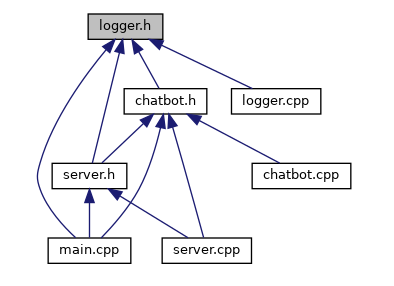
\includegraphics[width=0.8\textwidth]{include-graph-logger}
  \caption{Include graph-ul pentru clasa Logger.}
  \label{fig:includeGraphLogger}
\end{figure}

\subsection{Server}

În fișierul "Server.h" avem două clase, "MyRequestHandler" și "MyRequestHandlerFactory", care sunt wrappere peste clasele Poco::Net::HTTPRequestHandler și Poco::Net::HTTPRequestHandlerFactory. Aceste clase conțin logica necesară pentru a gestiona cererile și a furniza răspunsurile serverului.

La nivel top-level, avem următoarele funcționalități:

\begin{enumerate}
  \item Clasa "MyRequestHandler" este o clasă derivată din clasa Poco::Net::HTTPRequestHandler și reprezintă handler-ul care procesează cererile primite de la utilizatori. Metoda "handleRequest" primește cererea HTTP de la utilizator și verifică tipul acesteia. Dacă cererea este un payload JSON, atunci este mesajul trimis de utilizator prin JavaScript. Dacă conținutul este o cerere simplă pentru un fișier (sau legături către fișiere), atunci cererea este pasată metodei "serveResponse" pentru a trimite răspunsul (adică fișierul) corespunzător.

  \item Metoda "serveResponse" trimite prin răspuns fișierul solicitat de client sau o pagină HTML. Aceasta primește răspunsul HTTP și numele fișierului solicitat împreună cu extensia acestuia. Este necesară specificarea extensiei deoarece aceasta indică folderul în care se află fișierul.

  \item Clasa "MyRequestHandlerFactory" este o clasă derivată din clasa Poco::Net::HTTPRequestHandlerFactory și reprezintă o clasă de tip \emph{factory} de handler-e pentru fiecare cerere individuală. Metoda "createRequestHandler" creează un nou handler pentru fiecare cerere primită.
\end{enumerate}

Ambele clase utilizează obiectul "logger" din clasa "MyLogger" pentru a înregistra informații relevante și a le afișa în consolă sau a le scrie în fișiere de log.

Aceste wrapper-e peste clasele din biblioteca POCO oferă un nivel de abstractizare și encapsulare pentru a gestiona cererile primite de la utilizatori și a furniza răspunsurile corespunzătoare. Ele permit serverului să ofere un serviciu robust și scalabil, gestionând diferite tipuri de cereri și direcționându-le către funcționalitățile adecvate ale aplicației.

\begin{figure}[h]
  \centering
  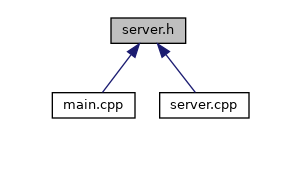
\includegraphics[width=0.6\textwidth]{include-graph-server}
  \caption{Include graph-ul pentru clasa Server.}
  \label{fig:includeGraphServer}
\end{figure}
\chapter{Concluzii}

În această lucrare de licență, am abordat implementarea și funcționarea unui chatbot utilizând Dialogflow, un serviciu dezvoltat de Google pentru înțelegerea limbajului natural și gestionarea conversațiilor. Chatbot-ul implementat are capacitatea de a interacționa cu utilizatorii într-un mod inteligent și de a oferi răspunsuri personalizate și relevante.

Am început prin a explora principiile de bază ale tehnologiei de chatbot și am identificat avantajele pe care le oferă, cum ar fi automatizarea proceselor, îmbunătățirea experienței utilizatorilor și creșterea eficienței operaționale. Am realizat o analiză a platformei Dialogflow și a funcționalităților sale, precum și a modului în care aceasta se integrează cu alte servicii și API-uri.

În continuare, am prezentat implementarea unui chatbot utilizând Dialogflow și Google Cloud Function. Am examinat modul în care se configurează un agent Dialogflow și cum se stabilesc intent-uri și întrebări de căutare pentru a ghida conversația cu utilizatorii. Am detaliat logica de procesare a cererilor și generare a răspunsurilor, inclusiv interacțiunea cu servicii externe pentru a obține informații sau a efectua operații specifice.

De asemenea, am explorat integrarea chatbot-ului cu un serviciu de stocare în cloud și modul în care acesta poate fi utilizat pentru a gestiona și accesa date specifice. Am prezentat exemple concrete de funcționalități implementate în chatbot, cum ar fi verificarea soldului conturilor bancare, transferul de bani, crearea și ștergerea de conturi.

În concluzie, această lucrare de licență a evidențiat potențialul și beneficiile implementării unui chatbot utilizând Dialogflow. Chatbot-ul oferă o modalitate eficientă și interactivă de a interacționa cu utilizatorii, facilitând gestionarea conversațiilor și furnizarea de răspunsuri personalizate. Implementarea chatbot-ului a implicat utilizarea unor tehnologii și servicii avansate, precum Dialogflow, Google Cloud Storage și Google Cloud Function, care au oferit un mediu puternic și scalabil pentru dezvoltarea și rularea chatbot-ului.

În viitor, există potențial pentru extinderea funcționalităților chatbot-ului și integrarea sa cu alte sisteme și platforme. De asemenea, se pot explora metode avansate de înțelegere a limbajului natural și de procesare a conversațiilor pentru a oferi o experiență și mai fluidă și personalizată utilizatorilor.

Implementarea și dezvoltarea unui chatbot reprezintă o provocare interesantă și promițătoare în domeniul inteligenței artificiale și al interacțiunii om-calculator. Prezenta lucrare a oferit oportunitatea de a explora această tehnologie și de a înțelege beneficiile și provocările implicate.

\begin{appendix}
% Pentru anexe
\end{appendix}

\printbibliography[heading=bibintoc]

\end{document}